\documentclass[11pt]{article}
\usepackage{graphicx}
\usepackage{amsmath}
\author{Ada Augusta, Countess of Lovelace}
\title{Notes By the Translator Upon the Memoir: Sketch of the Analytical Engine Invented
by Charles Babbage}
\date{October, 1842}
\begin{document}
\maketitle

\section{Note G}

\begin{figure}[htbp!]
\begin{center}
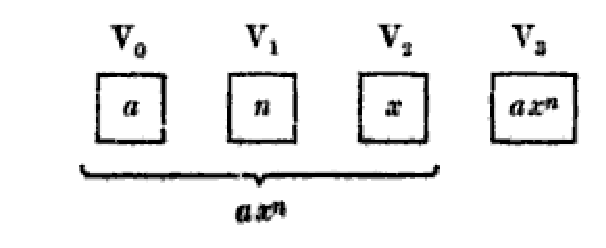
\includegraphics[width=0.5\textwidth]{var_diagram}
\end{center}
\caption{Any set of columns on which numbers are inscribed, represents merely a 
general function of the several quantities, until the special function have 
been impressed by means of the Operation and Variable-cards.}
\label{fig:var_diagram}
\end{figure}

The particular function whose integral the Difference Engine was constructed to
tabulate, is $\Delta^7u_x=0$. The purpose which that engine has been specially
intended and adapted to fulfil, is the computation of nautical and astronomical
tables. The integral of $\Delta^7u_x=0$ being   $u_z =
a+bx+cx^2+dx^3+ex^4+fx^5+gx^6$, the constants a, b, c, etc. are represented on the
seven columns of discs, of which the engine consists.

\pagebreak
The following is a more complicated example of the manner in which the
engine would compute a trigonometrical function containing variables.
To multiply

\begin{align}
&A+A_1 \cos \theta + A_2\cos 2\theta + A_3\cos 3\theta + \cdots
\intertext{by}
&B + B_1 \cos \theta.
\end{align}


\nocite{*}

\bibliographystyle{plain}
\bibliography{refs}

\end{document}
